
%(BEGIN_QUESTION)
% Copyright 2006, Tony R. Kuphaldt, released under the Creative Commons Attribution License (v 1.0)
% This means you may do almost anything with this work of mine, so long as you give me proper credit

Et stort vannfilter tettes av og til av partikler, og drift ønsker en indikasjon på dette.  Siden tetting av filteret gir større differansetrykk over filteret ved gitt vannstrøm, vil måling med differansetrykkmanometer gi en enkel indikator på tetting.

Tegn tilkoblingsrørene mellom differansetrykkmåleren og filteret (de to ``taps'' på rørene er klare for instrumentrør), slik at måleren viser positivt trykk når filteret tettes:

$$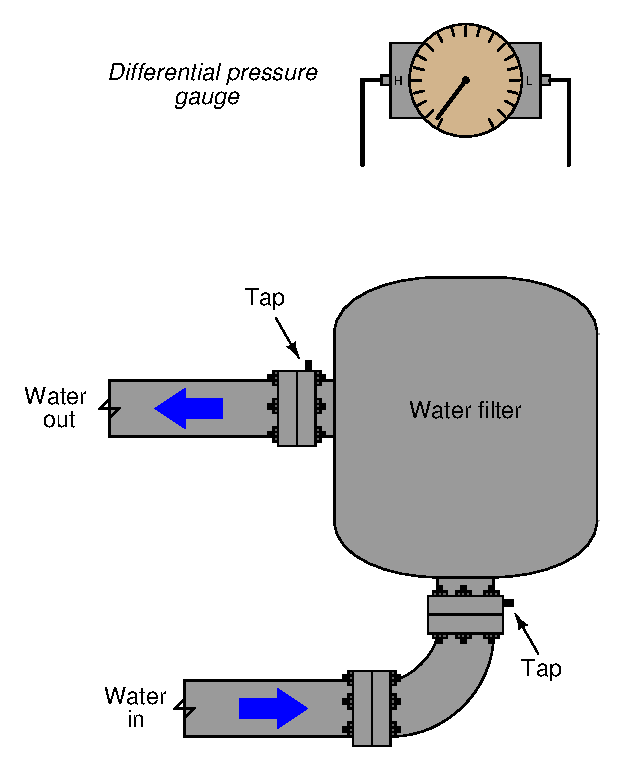
\includegraphics[width=15.5cm]{i00215x01.eps}$$

\underbar{file i00215}
%(END_QUESTION)





%(BEGIN_ANSWER)


%(END_ANSWER)





%(BEGIN_NOTES)

For korrekt tilkobling kobles ``high''-siden til oppstrøms tap (``water in''), og ``low''-siden til nedstrøms tap (``water out'').

\vskip 10pt

Dette velges fordi oppstrøms side av en struping alltid har høyere trykk enn nedstrøms side, og ved økende filtertetting ønsker du økende målerindikasjon.  Koble derfor målerens ``high'' til siden som øker mest i trykk ved tetting, og ``low'' til siden som forblir lavere.

%INDEX% Measurement, pressure: using a D/P cell for filter plugging detection
%INDEX% Process: water filter (generic)

%(END_NOTES)

